%%%%%%%%%% DOCUMENT STUFF %%%%%%%%%%

\documentclass[10.5pt,letterpaper]{article}
\usepackage{mathtools}
\usepackage{amsmath}
\usepackage{amssymb}
\usepackage{datetime}
\usepackage{setspace}
\usepackage{tikz}
\usepackage[margin=1in]{geometry}
\usepackage{courier}
\usepackage{listings}
\usepackage{mips}
\usepackage{graphicx}
\usepackage{enumitem}
\usepackage{pgfplots}
\usepackage{colortbl}
\usepackage{mdframed}
\usepackage{xcolor}

%%%%%%%%%% FORMATTING %%%%%%%%%%

\newdate{date}{26}{11}{2017}
\spacing{1.5}
\date{\displaydate{date}}
\setcounter{secnumdepth}{0}
\newcommand\tab[1][0.5cm]{\hspace*{#1}}
\newcommand*\circled[1]{\tikz[baseline=(char.base)]{
            \node[shape=circle,draw,inner sep=2pt] (char) {#1};}}
\lstset{language=[mips]Assembler}
\usetikzlibrary{arrows,shapes,automata,petri,positioning,calc}

\tikzset{
    place/.style={
        circle,
        thick,
        draw=black,
        minimum size=6mm,
    },
        state/.style={
        circle,
        thick,
        draw=black!75,
        %fill=green!20,
        minimum size=6mm,
    },
}

\graphicspath{{images/}}

%%%%%%%%%% CONTENT %%%%%%%%%%

%%%%% COVER PAGE %%%%%

\begin{document}
\title{CS 161: Homework 7}
\author{
	Jonathan Woong\\
	804205763\\
	Fall 2017\\
	Discussion 1A}
\maketitle
\pagebreak

%%%%% PROBLEMS %%%%%

\begin{enumerate}[label=\textbf{Problem \arabic*.}]
\item Prove:
	\begin{enumerate}[label=\alph*)]
	\item Generalized product rule: $Pr(A,B|K) = Pr(A|B,K)Pr(B|K)$
	\begin{equation}\nonumber\begin{split}
	Pr(A,B|K) &= \frac{Pr(A,B,K)}{Pr(B|K)} \\
	&= \frac{Pr(A|B,K)Pr(B,K)}{Pr(K)}\\
	&= \frac{Pr(A|B,K)Pr(B|K)Pr(K)}{Pr(K)}\\
	&= Pr(A|B,K)Pr(B|K)\\
	\end{split}\end{equation}
	\item Generalized Bayes' rule: $Pr(A|B,K) = \frac{Pr(B|A,K)Pr(A|K)}{Pr(B|K)}$
	\begin{equation}\nonumber\begin{split}
	Pr(A|B,K) &= \frac{Pr(A,B|K)}{Pr(B|K)}\\
	&= \frac{Pr(A,B,K)}{\frac{Pr(K)}{Pr(B|K)}}\\
	&= \frac{Pr(B|A,K)Pr(A,K)}{\frac{Pr(K)}{Pr(B|K)}}\\
	&= \frac{Pr(B|A,K)Pr(A|K)}{Pr(B|K)}\\
	\end{split}\end{equation}
	\end{enumerate}
\item We have a bag of three biased coins a, b, and c with probabilities of coming up heads of 20\%, 60\%, and 80\% respectively. One coin is drawn randomly from the bag (with equal likelyhood of drawing each of the three coins), and then the coin is flipped three times to generate the outcones $X_1$, $X_2$, and $X_3$.\\
Draw the Bayesian network corresponding to this setup and define the necessary CPTs (Conditional Probability Table).\\
Let $C$ be the random variable representing the coin that we drew:
\[\begin{tabular}{|c|c|}
\hline
$C$ & $Pr(C)$ \\
\hline
a & $\frac{1}{3}$ \\
\hline
b & $\frac{1}{3}$ \\
\hline
c & $\frac{1}{3}$ \\
\hline
\end{tabular}\tab
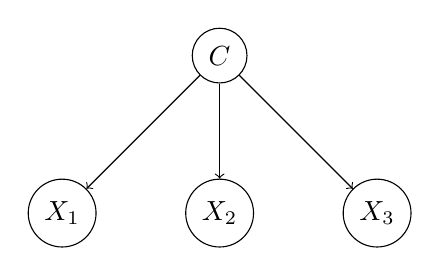
\begin{tikzpicture}
\node[shape=circle,draw=black](C) at (2,0) {$C$};
\node[shape=circle,draw=black](X1) at (0,-2) {$X_1$};
\node[shape=circle,draw=black](X2) at (2,-2) {$X_2$};
\node[shape=circle,draw=black](X3) at (4,-2) {$X_3$};
\path[->] (C) edge node {} (X1);
\path[->] (C) edge node {} (X2);
\path[->] (C) edge node {} (X3);
\end{tikzpicture}\]
The CPT for any $X_i$ is given below:
\[\begin{tabular}{|c|c|c|}
\hline
$C$ & $X_i$ & $Pr(X_i|C)$ \\
\hline
a & heads & 0.2 \\
\hline
a & tails & 0.8 \\ 
\hline
b & heads & 0.6 \\
\hline
b & tails & 0.4 \\
\hline
c & heads & 0.8 \\
\hline
c & tails & 0.2 \\
\hline
\end{tabular}\]
\item Consider the set of objects below.\\
\tikz \node[draw=black,color=black,fill=gray]{1};
\tikz \node[draw=black,color=black,fill=gray]{1};
\tikz \node[draw=black,color=black,fill=gray]{2};
\tikz \node[draw=black,color=black,fill=gray]{2};
\tikz \node[draw=black,color=black,fill=gray]{2};
\tikz \node[draw=black,color=black,fill=gray]{2};
\tikz \node[draw=black,circle,color=black,fill=gray,scale=0.75]{1};
\tikz \node[draw=black,circle,color=black,fill=gray,scale=0.75]{2};
\tikz \node[draw=black,circle,color=black,fill=gray,scale=0.75]{2};\\
\boxed{1} \boxed{2} \circled{1} \circled{2}\\
Mr. Y picked up an object at random from the above set. We want to compute the probabilty of the following events:
	\begin{enumerate}[label=$\alpha_\arabic*$:]
	\item the object is black;
	\item the object is square;
	\item if the object is one or black, then it is also square.
	\end{enumerate}
Construct the joint probability distribution of this problem. Use it to compute the above probabilities by explicitly identifying the worlds at which each $\alpha_i$ holds. Identify two sets of sentences $\alpha,\beta,\gamma$ such that $\alpha$ is independent of $\beta$ given $\gamma$ with respect to the constructed distribution.
	\[\begin{tabular}{|c|c|c|c|c|c|}
	\hline
	world & $Black$ & $Square$ & $One$ & count & probability \\
	\hline
	1 & T & T & T & 2 & 0.1538 \\
	\hline
	2 & T & T & F & 4 & 0.3077 \\
	\hline
	3 & T & F & T & 1 & 0.0769 \\
	\hline
	4 & T & F & F & 2 & 0.1538 \\
	\hline
	5 & F & T & T & 1 & 0.0769 \\
	\hline
	6 & F & T & F & 1 & 0.0769 \\
	\hline
	7 & F & F & T & 1 & 0.0769 \\
	\hline
	8 & F & F & F & 1 & 0.0769 \\
	\hline
	\end{tabular}\]
	\begin{enumerate}[label=$\alpha_\arabic*$:]
	\item holds for worlds 1, 2, 3, 4 
		\[Pr(\alpha_1)=0.1538+0.3077+0.0769+0.1538=\boxed{0.6922}\]
	\item holds for worlds 1, 2, 5, 6
		\[Pr(\alpha_2)=0.1538+0.3077+0.0769+0.7069=\boxed{0.6153}\]
	\item holds for worlds 1, 2, 5
		\[Pr(\alpha_3)=0.1538+0.3077+0.0769=\boxed{0.5384}\]
	\end{enumerate}
	\begin{enumerate}[label=\arabic*)]
	\item \fbox{$\alpha = One, \beta = Square, \gamma = Black$: 
		One is independent of Square given Black}\\
	$Pr(One|Black) = \frac{1}{3}$\\
	$Pr(One|Black,Square) = \frac{2}{6} = \frac{1}{3}$\\
	$Pr(One|Black) \equiv Pr(One|Black,Square) \implies \text{independence}$
	\item \fbox{$\alpha = One, \beta = Square, \gamma = \lnot Black$: 
		One is independent of Square given White}\\
	$Pr(One|\lnot Black) = \frac{1}{2}$\\
	$Pr(One|\lnot Black,Square) = \frac{1}{2}$\\
	$Pr(One|\lnot Black) \equiv Pr(One|\lnot Black,Square) \implies \text{independence}$
	\end{enumerate} 
\item Consider the DAG:
\[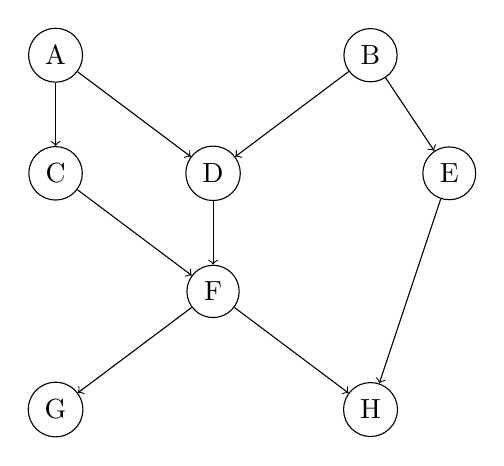
\begin{tikzpicture}
	\node[shape=circle,draw=black](A) at (0,0) {A};
	\node[shape=circle,draw=black](B) at (4,0) {B};
	\node[shape=circle,draw=black](C) at (0,-1.5) {C};
	\node[shape=circle,draw=black](D) at (2,-1.5) {D};
	\node[shape=circle,draw=black](E) at (5,-1.5) {E};
	\node[shape=circle,draw=black](F) at (2,-3) {F};
	\node[shape=circle,draw=black](G) at (0,-4.5) {G};
	\node[shape=circle,draw=black](H) at (4,-4.5) {H};
	\path[->](A) edge node {} (C)
		edge node {} (D);
	\path[->](B) edge node {} (D)
		edge node {} (E);
	\path[->](C) edge node {} (F);
	\path[->](D) edge node {} (F);
	\path[->](E) edge node {} (H);
	\path[->](F) edge node {} (G)
		edge node {} (H);
\end{tikzpicture}\]
	\begin{enumerate}[label=(\alph*)]
	\item List the Markovian assumptions asserted by the DAG.
	\begin{enumerate}[label=\arabic*)]
	\item $I(A,\emptyset,\{B,E\})$
	\item $I(B,\emptyset,\{A,C\})$
	\item $I(C,A,\{B,D,E\})$
	\item $I(D,\{A,B\},\{C,E\})$
	\item $I(E,B,\{A,C,D,F,G\})$
	\item $I(F,\{C,D\},\{A,B,E\})$
	\item $I(G,F,\{A,B,C,D,E,H\})$
	\item $(H,\{E,F\},\{A,B,C,D,G\})$
	\end{enumerate}
	\item True or false? Why?
		\begin{itemize}
			\item $d\_separated(A,BH,E)$: \fbox{False, there exists a path $A\rightarrow C \rightarrow F \rightarrow H \rightarrow E$}
			\item $d\_separated(G,D,E)$: \fbox{False, there exists a path $G \rightarrow F \rightarrow H \rightarrow E$}
			\item $d\_separated(AB,F,GH)$: \fbox{False, there exists a path $B \rightarrow E \rightarrow H$}
		\end{itemize}
	\item Express $Pr(a,b,c,d,e,f,g,h)$ in factored form using the chain rule for Bayesian networks.
	\begin{equation}\nonumber\begin{split}
	Pr(a,b,c,d,e,f,g,h) &= Pr(a|b,c,d,e,f,g,h) \times \\
	& Pr(b|c,d,e,f,g,h) \times \\
	& Pr(c|d,e,f,g,h) \times \\
	& Pr(d|e,f,g,h) \times \\
	& Pr(e|f,g,h) \times \\
	& Pr(f|g,h) \times \\
	& Pr(g|h) \times \\
	& Pr(h) \\
	\end{split}\end{equation}
	\item Compute $Pr(A=0,B=0)$ and $Pr(E=1|A=1)$. Justify your answers.
	\end{enumerate}
	\begin{tabular}{|c|c|}
	\hline
	$Pr(A=0)$ & $Pr(A=1)$ \\
	\hline
	0.8 & 0.2 \\
	\hline
	\end{tabular}
	\begin{tabular}{|c|c|}
	\hline
	$Pr(B=0)$ & $Pr(B=1)$ \\
	\hline
	0.3 & 0.7 \\
	\hline
	\end{tabular}\\
	\begin{tabular}{|c|c|c|}
	\hline
	& $Pr(E=0|B)$ & $Pr(E=1|B)$ \\
	\hline
	$B=0$ & 0.1 & 0.9 \\
	\hline
	$B=1$ & 0.9 & 0.1 \\
	\hline
	\end{tabular}\\
	\begin{tabular}{|c|c|c|}
	\hline
	& $Pr(D=0|A,B)$ & $Pr(D=1|A,B)$ \\
	\hline
	$A=0,B=0$ & 0.2 & 0.8 \\
	\hline
	$A=0,B=1$ & 0.9 & 0.1 \\
	\hline
	$A=1,B=0$ & 0.4 & 0.6 \\
	\hline
	$A=1,B=1$ & 0.5 & 0.5 \\
	\hline
	\end{tabular}
	\begin{enumerate}[label=\arabic*)]
		\item $Pr(A=0,B=0)$\\
		Since $A$ and $B$ are independent: \\
		\begin{equation}\nonumber\begin{split}
		Pr(A=0,B=0) &= Pr(A=0)Pr(B=0)\\
		&= (0.8)(0.3)\\
		&= \boxed{0.24}
		\end{split}\end{equation}
		\item $Pr(E=1|A=1)$\\
		Since $E$ and $A$ are independent: \\
		\begin{equation}\begin{split}
		Pr(E=1|A=1) &= Pr(E=1)\\
		&= Pr(E=1|B=0)Pr(B=0) + Pr(E=1|B=1)Pr(B=1)\\
		&= (0.9)(0.3) + (0.1)(0.7)\\
		&= 0.07 + 0.27\\
		&= \boxed{0.34}
		\end{split}\end{equation}
	\end{enumerate}
\end{enumerate}
\end{document}